\scanpage{64}
\begin{center}
U N I V E R S I T E\\
DES SCIENCES ET TECHNIQUES\\
\uline{DU LANGUEDOC}\\
MR/MD
\end{center}
Diffusion : Liste A\\
n\textdegree\ 4172

Montpellier, le 3 juillet 1978

\begin{center}
AVIS DE SOUTENANCE D'UNE THESE DE DOCTORAT DE SPECIALITE

\uline{SCIENCES BIOLOGIQUES} - \uline{Mention ECOLOGIE}
\end{center}

\uline{Nom et prénom du candidat} : LIVET François

\uline{Titre de la thèse} : L'herpétofaune du nord-ouest de la Montagne Noire.
Biogéographie et écologie.

\uline{Date, heure et lieu de soutenance prévus} : Jeudi 6 juillet à 8 heures -
amphithéâtre 9

\uline{Nom du Directeur de thèse} : Monsieur J. BONS

\uline{Désignation du laboratoire où la thèse est préparée} : Laboratoire de bio-\\
géographie et écologie des vertébrés E.P.H.E.

\uline{Analyse de l'ouvrage} : Le peuplement des Amphibiens et Reptiles de la Montagne
Noire a été analysé en tenant compte des milieux qui les hébergent.
Différents indices, probabilité de présence, diversité spécifique, richesse
spécifique ont été calculés et permettent de classer les milieux naturels.
L'impact humain sur certaines espèces d'Ophidiens a pu être envisagé.

\uline{Durée approximative des recherches ayant abouti à la thèse} : 3 ans

\uline{Composition du jury} :
\diagram{\(\begin{array}{l}
\text{M. R. LEGENDRE, Président}\\
\text{M. M. GODRON}\\
\text{M. J. BONS}\\
\text{M. G. PASTEUR}
\end{array}\)}

Le Secrétaire Général,

\figure{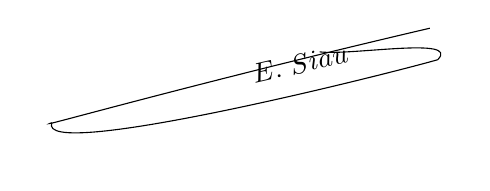
\begin{tikzpicture}
\draw (-2.7,-0.7) .. controls (-3,-0.8) and (-0.9,-0.2) .. (2.1,0.5);
\draw (-2.7,-0.7) .. controls (-2.9,-1.2) and (1.5,-0.1) .. (2.2,0.1)
.. controls (2.5,0.4) and (1.1,0.15) .. (0.7,0.2);
\node[rotate=13] at (0.45,0.05) {\(\unsure{E.\ Siau}\)};
\end{tikzpicture}}

\uline{E. SIAU}
\mspage{63}

